\chapter*{Anhang}
\section*{CCSS Mathe Abhängigkeitsbaum}
	\label{CCSSMath}
	\begin{center}
		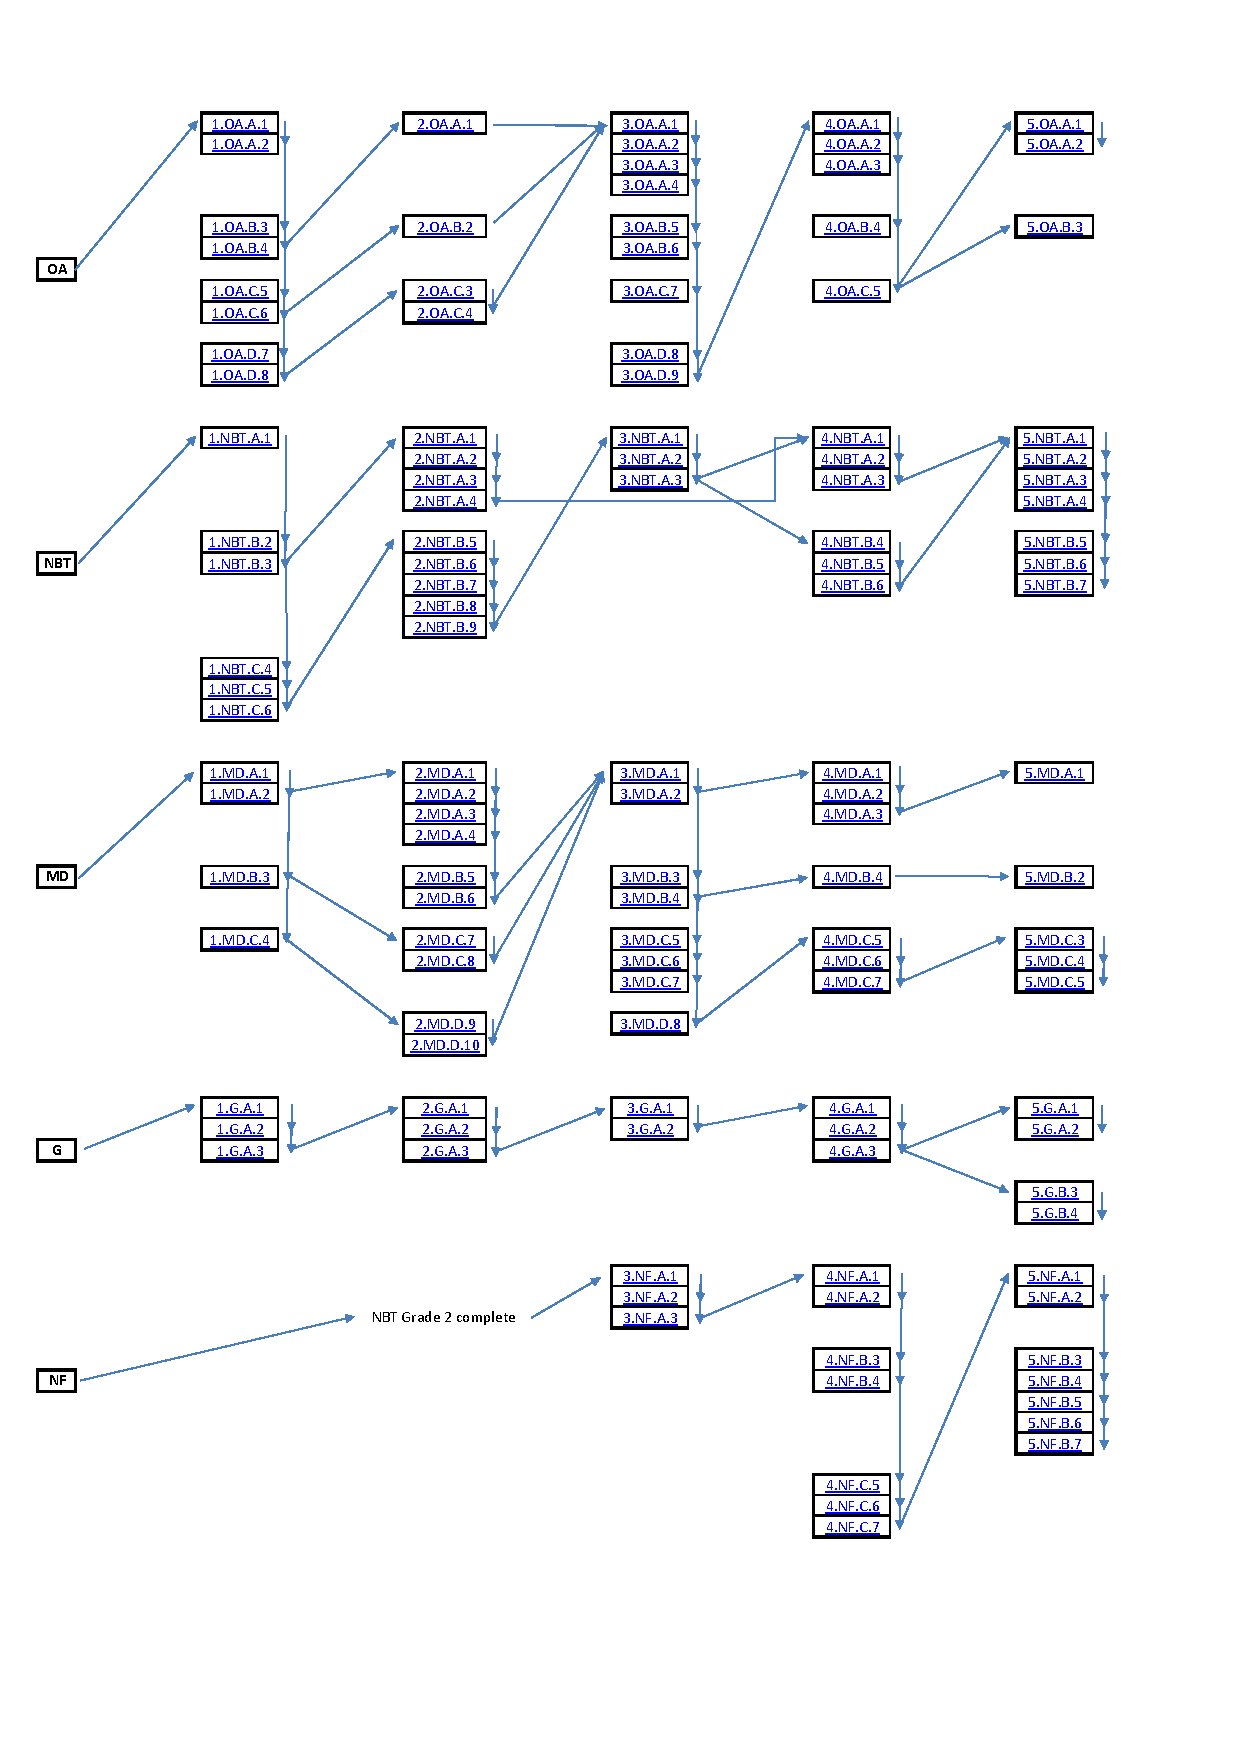
\includepdf[pages={1-},scale=1]{pics/CCSS-Math.pdf}
	\end{center}

\section*{CCSS Englisch Abhängigkeitsbaum}
	\label{CCSSEnglish}
	\begin{center}
		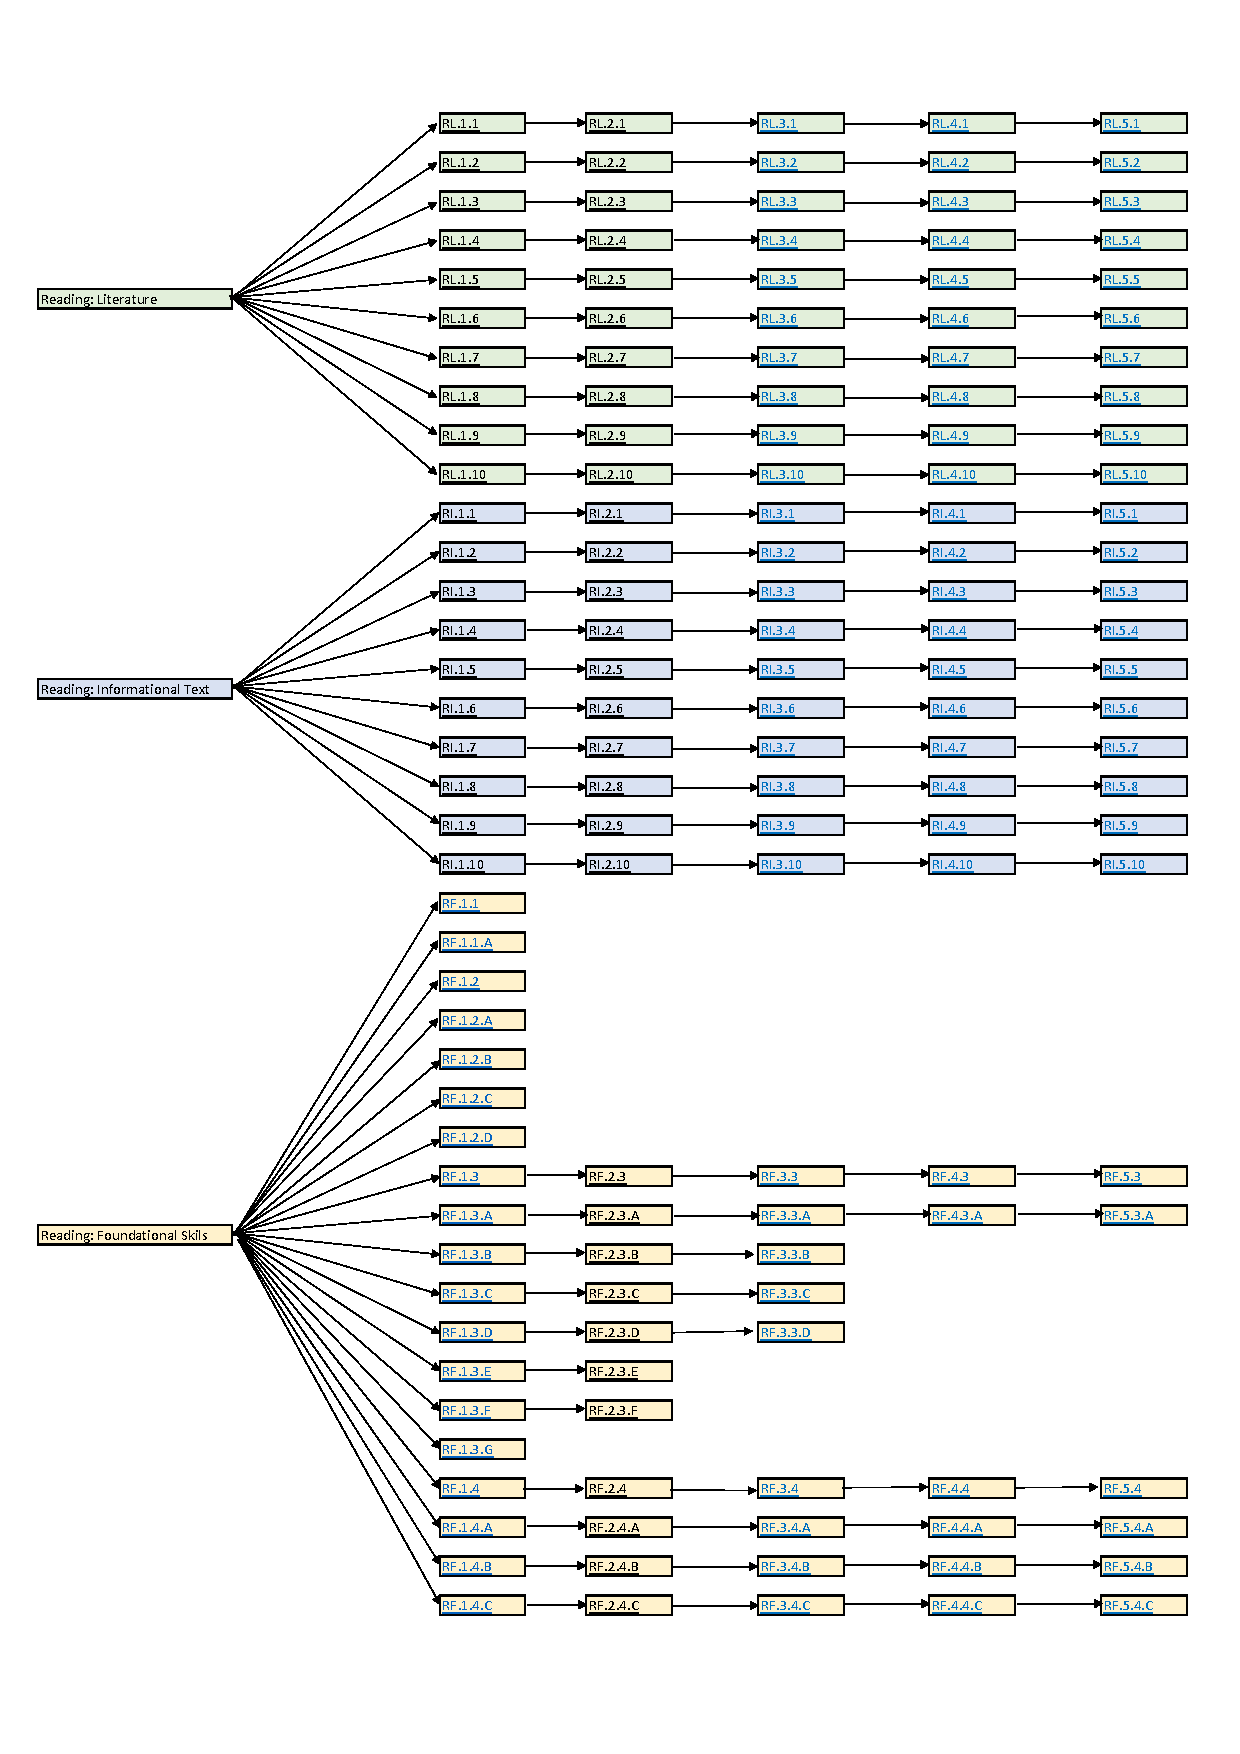
\includepdf[pages={1-},scale=1]{pics/CCSS-English.pdf}
	\end{center}
	
\section*{Usability Evaluation}
	\label{UEMarcel}
	\begin{center}
		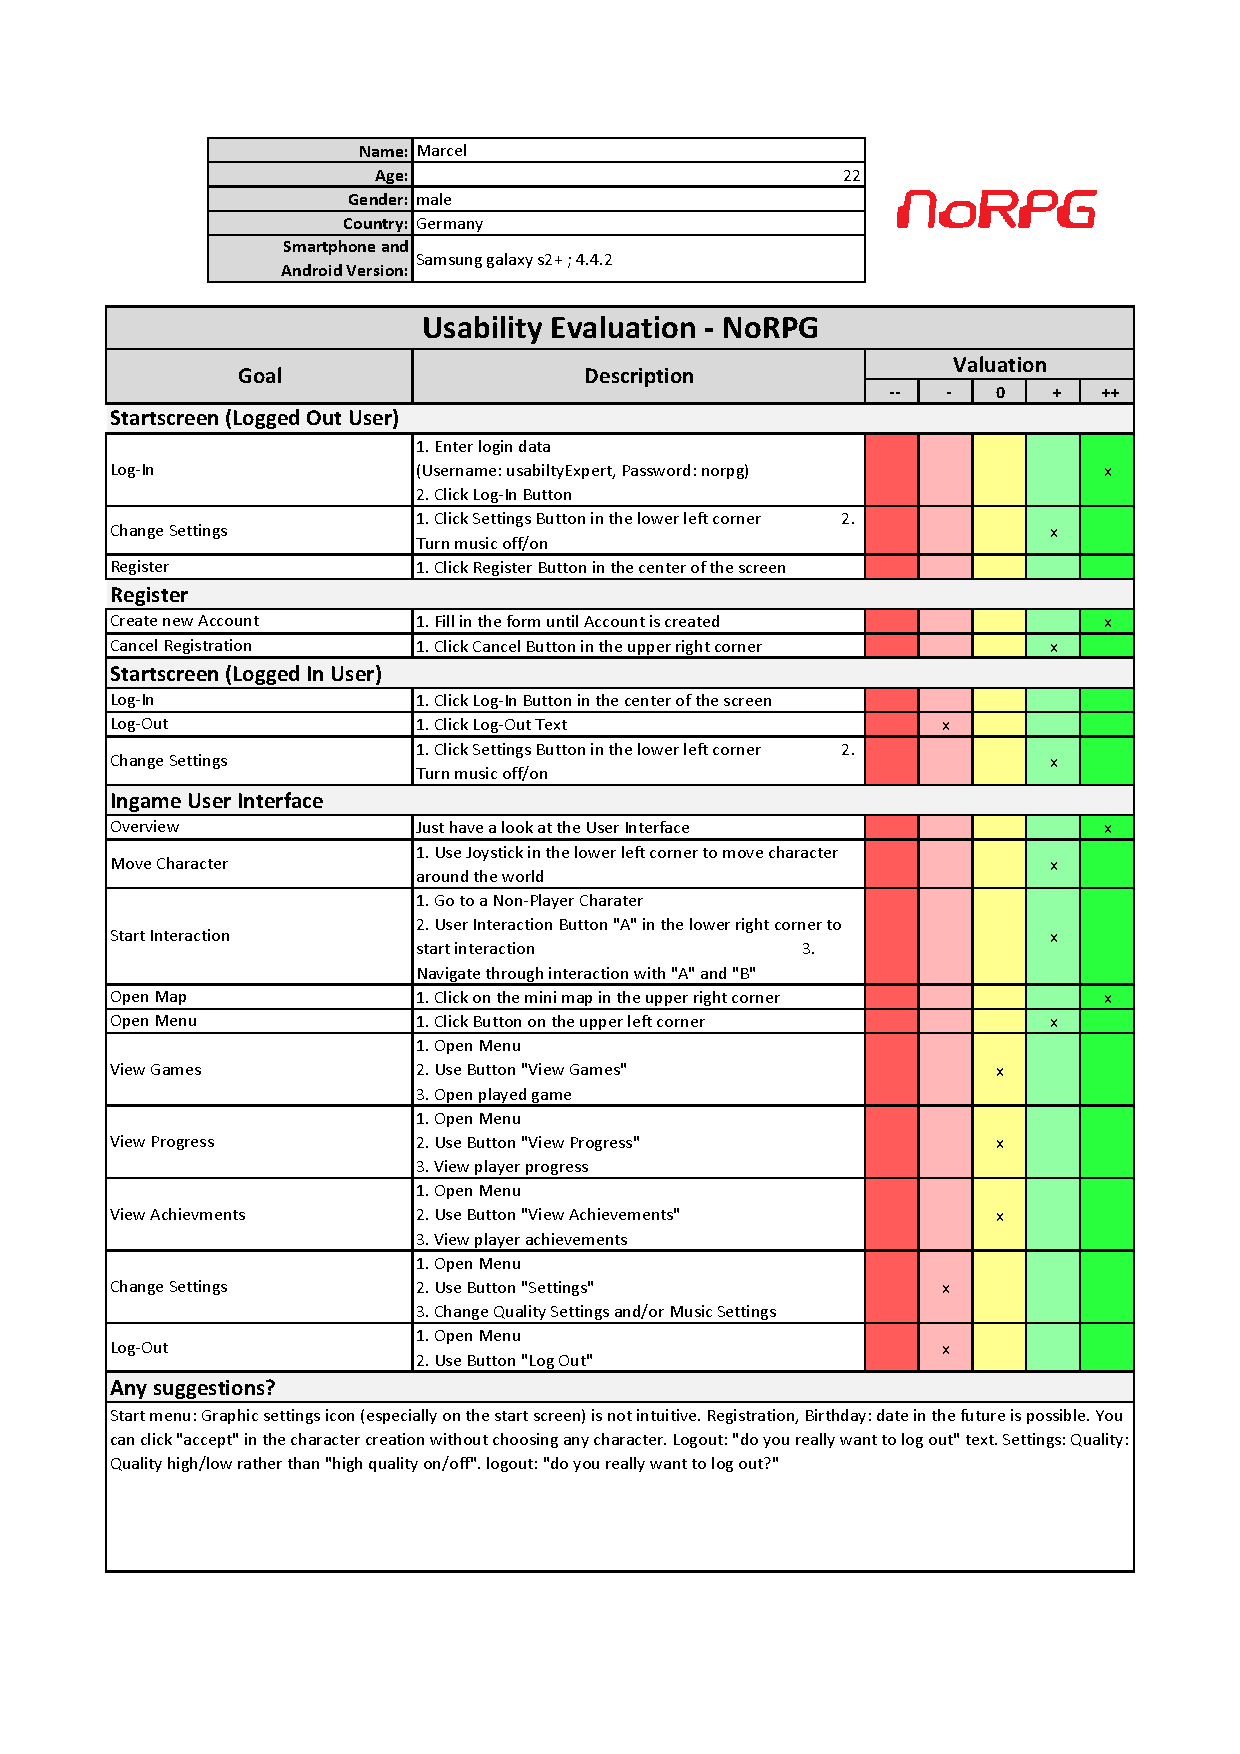
\includepdf[pages={1-},scale=1]{pics/UE-Marcel.pdf}
	\end{center}
\section*{Skripte für die Datenhaltung}
	\label{anhang4}

\begin{scriptsize}
				\lstset{
					float,
					caption=LoadingScreen.cs, 
					language=[Sharp]C, 
					frame=single,  
					showstringspaces=false, 
					showspaces=false, 
					numbers=left, 
					captionpos=b, 
					belowcaptionskip=4pt,
					basicstyle=\ttfamily
				} 
				\begin{lstlisting}[label=lst:methode34]
using UnityEngine;
using UnityEngine.SceneManagement;

public class LoadingScreen : MonoBehaviour {
    private static bool isInitialized = false;

    public static MappingStandardsToCourses Settings {
        get; private set;
    }

    private static void Initialize() {
        if (isInitialized) {
            return;
        }

        IConfigReader configReader = new WebJSONConfigReader();
        Settings = configReader.LoadSettings();

        isInitialized = true;
    }

    public void Start() {
        Initialize();

    }
}
				\end{lstlisting}
			\end{scriptsize}

\begin{scriptsize}
				\lstset{
					float,
					caption=IConfigReader.cs, 
					language=[Sharp]C, 
					frame=single,  
					showstringspaces=false, 
					showspaces=false, 
					numbers=left, 
					captionpos=b, 
					belowcaptionskip=4pt,
					basicstyle=\ttfamily
				} 
				\begin{lstlisting}[label=lst:methode35]
interface IConfigReader {
    MappingStandardsToCourses LoadSettings();
}


				\end{lstlisting}
			\end{scriptsize}
			
\begin{scriptsize}
				\lstset{
					float,
					caption=MappingStandardsToCoursesBean.cs, 
					language=[Sharp]C, 
					frame=single,  
					showstringspaces=false, 
					showspaces=false, 
					numbers=left, 
					captionpos=b, 
					belowcaptionskip=4pt,
					basicstyle=\ttfamily
				} 
				\begin{lstlisting}[label=lst:methode3]
using System;
using UnityEngine;

[Serializable]
public class MappingStandardsToCoursesBean {
    public ClassBean[] classes;

    public static MappingStandardsToCoursesBean CreateFromJSON(string json) {
        return JsonUtility.FromJson<MappingStandardsToCoursesBean>(json);
    }
}

[Serializable]
public class ClassBean {
    public string name;
    public CourseBean[] courses;
}

[Serializable]
public class CourseBean {
    public string name;
    public StandardBean[] standards;
}

[Serializable]
public class StandardBean {
    public string name;
    public string[] vorbedingungen;
    public string[] nachbedingungen;
    public GamesBean[] games;
}

[Serializable]
public class GamesBean {
    public string id;
    public string name;
    public string url;
    public string standard;
}


				\end{lstlisting}
			\end{scriptsize}

\begin{scriptsize}
				\lstset{
					float,
					caption=MappingStandardsToCourses.cs, 
					language=[Sharp]C, 
					frame=single,  
					showstringspaces=false, 
					showspaces=false, 
					numbers=left, 
					captionpos=b, 
					belowcaptionskip=4pt,
					basicstyle=\ttfamily
				} 
				\begin{lstlisting}[label=lst:methode3]
public class MappingStandardsToCourses {
    public readonly Classes[] classes;
    public MappingStandardsToCourses(Classes[] classes) {
        this.classes = classes;
    }
}

public class Classes {
    public readonly Courses[] courses;
    public readonly string name; 

    public Classes(string name, Courses[] courses) {
        this.name = name; 
        this.courses = courses; 
    }
}

public class Courses {
    public readonly Standards[] standards;
    public readonly string name; 

    public Courses(string name, Standards[] standards) {
        this.name = name;
        this.standards = standards;
    }
}
    
public class Standards {
    public readonly string name;
    public readonly string[] vorbedingungen;
    public readonly string[] nachbedingungen;
    public readonly Games[] games;

    public Standards(string name, string[] vorbedingungen, 
    	string[] nachbedingungen, Games[] games) {
        this.name = name; 
        this.nachbedingungen = nachbedingungen;
        this.vorbedingungen = vorbedingungen; 
        this.games = games;
    }
}

[System.Serializable]
public class Games {
    public readonly string id;
    public readonly string name;
    public readonly string url;
    private string standard;

    public Games(string id, string name, string url) {
        this.name = name;
        this.id = id;
        this.url = url;
        this.standard = "";
    }

    public string Standard {
        get {
            return standard;
        }

        set {
            standard = value;
        }
    }
}
				\end{lstlisting}
			\end{scriptsize}